\documentclass[border=5pt]{standalone}
\usepackage[T1]{fontenc}
\usepackage{lmodern}
\usepackage{pgfplots}
\usepgfplotslibrary{groupplots}
\pgfplotsset{compat=1.18}
\begin{document}\sffamily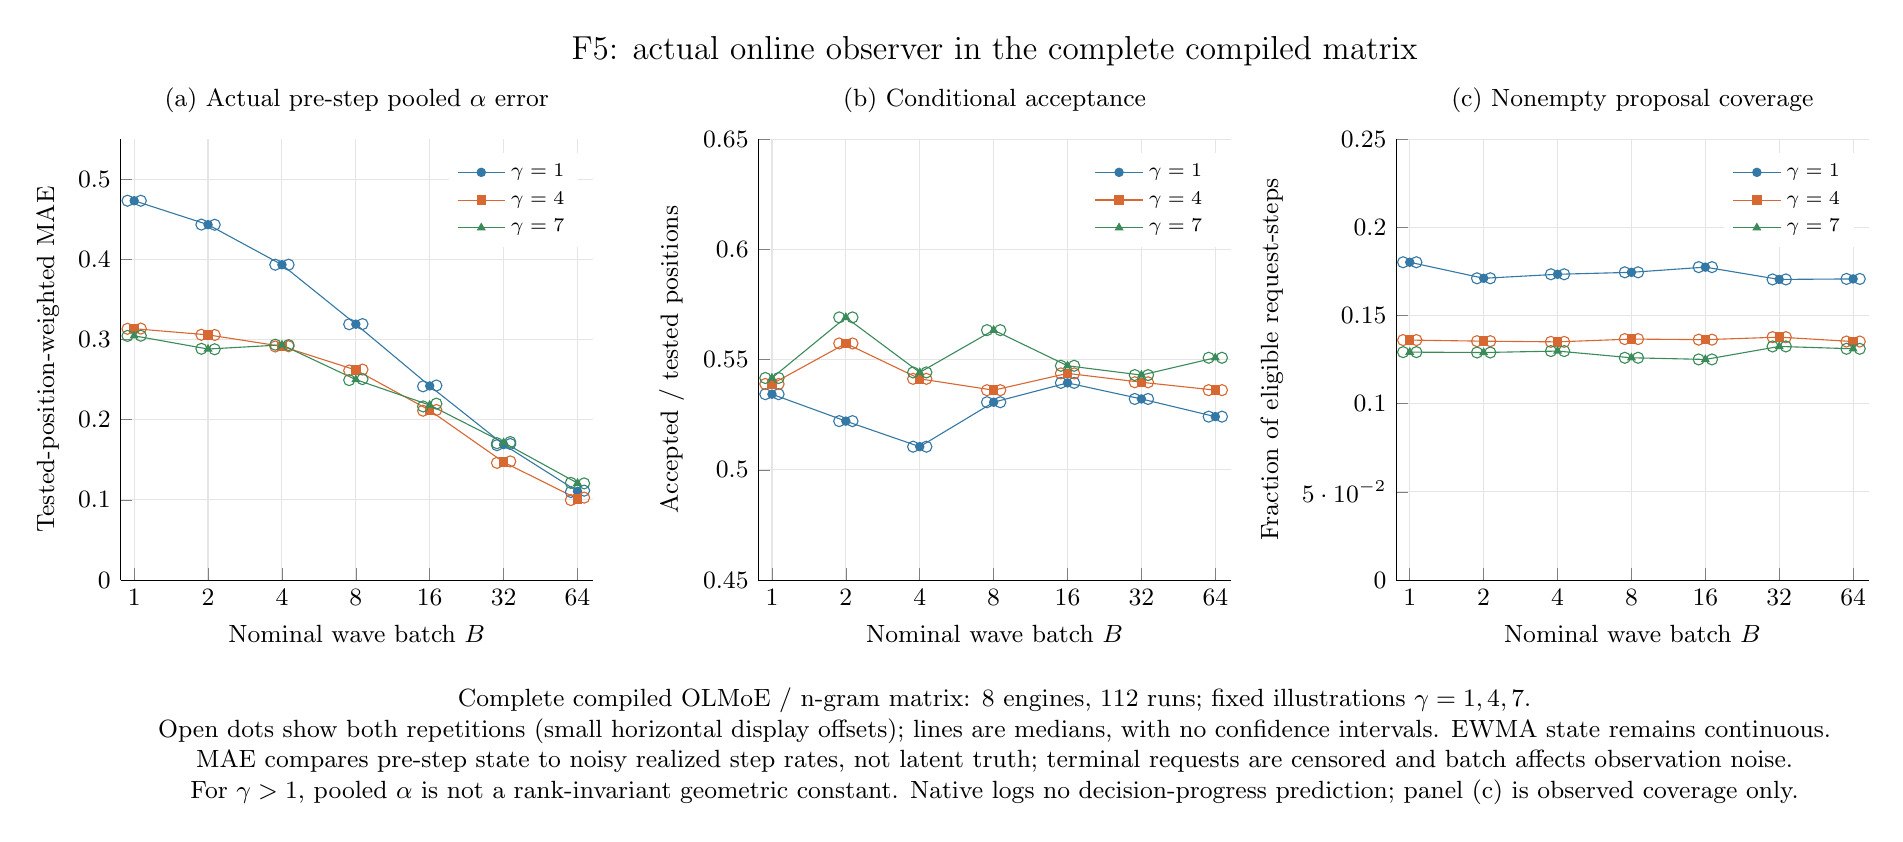
\begin{tikzpicture}
\definecolor{cal}{HTML}{3478A5}\definecolor{test}{HTML}{D76832}\definecolor{profile}{HTML}{3B8A5A}
\begin{groupplot}[group style={group size=3 by 1,horizontal sep=2.1cm},width=6.0cm,height=5.6cm,scale only axis,axis lines*=left,grid=major,grid style={gray!20},tick label style={font=\small},label style={font=\small},title style={font=\small},legend style={font=\scriptsize,draw=none},unbounded coords=jump]
\nextgroupplot[title={(a) Actual pre-step pooled $\alpha$ error},ylabel={Tested-position-weighted MAE},ymin=0,ymax=0.55,xmode=log,log basis x=2,xtick={1,2,4,8,16,32,64},xticklabels={1,2,4,8,16,32,64},xlabel={Nominal wave batch $B$},xmin=0.88,xmax=74,legend pos=north east]\addplot[color=cal,mark=*,mark size=1.5pt] coordinates {(1,0.473223159184) (2,0.44336839148) (4,0.393423865496) (8,0.319249232268) (16,0.242226312074) (32,0.169070568433) (64,0.110738591686)};
\addlegendentry{$\gamma=1$}
\addplot[forget plot,only marks,color=cal,mark=o,mark size=2pt,mark options={fill=white}] coordinates {(0.939522749214,0.473233180343) (1.87904549843,0.443473018344) (3.75809099686,0.393406755364) (7.51618199371,0.319146029062) (15.0323639874,0.241705941426) (30.0647279748,0.168328428915) (60.1294559497,0.109895589718) (68.119691677,0.111581593653) (34.0598458385,0.169812707951) (17.0299229193,0.242746682723) (8.51496145963,0.319352435475) (4.25748072981,0.393440975629) (2.12874036491,0.443263764616) (1.06437018245,0.473213138025)};
\addplot[color=test,mark=square*,mark size=1.5pt] coordinates {(1,0.313617023213) (2,0.305905736219) (4,0.291566663999) (8,0.262031021624) (16,0.211758679714) (32,0.147174266458) (64,0.101374697267)};
\addlegendentry{$\gamma=4$}
\addplot[forget plot,only marks,color=test,mark=o,mark size=2pt,mark options={fill=white}] coordinates {(0.939522749214,0.313495093869) (1.87904549843,0.306016906775) (3.75809099686,0.291430427059) (7.51618199371,0.261440455462) (15.0323639874,0.211292564721) (30.0647279748,0.146251510597) (60.1294559497,0.099846829797) (68.119691677,0.102902564736) (34.0598458385,0.148097022319) (17.0299229193,0.212224794706) (8.51496145963,0.262621587785) (4.25748072981,0.291702900938) (2.12874036491,0.305794565664) (1.06437018245,0.313738952557)};
\addplot[color=profile,mark=triangle*,mark size=1.5pt] coordinates {(1,0.30475554323) (2,0.28823394604) (4,0.293422795396) (8,0.250092190636) (16,0.218359886201) (32,0.171523953251) (64,0.120977129111)};
\addlegendentry{$\gamma=7$}
\addplot[forget plot,only marks,color=profile,mark=o,mark size=2pt,mark options={fill=white}] coordinates {(0.939522749214,0.304633338654) (1.87904549843,0.288541161248) (3.75809099686,0.293676762633) (7.51618199371,0.249471961834) (15.0323639874,0.216624594798) (30.0647279748,0.170794813443) (60.1294559497,0.12129786681) (68.119691677,0.120656391413) (34.0598458385,0.172253093059) (17.0299229193,0.220095177603) (8.51496145963,0.250712419438) (4.25748072981,0.29316882816) (2.12874036491,0.287926730831) (1.06437018245,0.304877747806)};
\nextgroupplot[title={(b) Conditional acceptance},ylabel={Accepted / tested positions},ymin=0.45,ymax=0.65,xmode=log,log basis x=2,xtick={1,2,4,8,16,32,64},xticklabels={1,2,4,8,16,32,64},xlabel={Nominal wave batch $B$},xmin=0.88,xmax=74,legend pos=north east]\addplot[color=cal,mark=*,mark size=1.5pt] coordinates {(1,0.534339622642) (2,0.522116903633) (4,0.510522213562) (8,0.530691530692) (16,0.539463601533) (32,0.532168387609) (64,0.52414885194)};
\addlegendentry{$\gamma=1$}
\addplot[forget plot,only marks,color=cal,mark=o,mark size=2pt,mark options={fill=white}] coordinates {(0.939522749214,0.534339622642) (1.87904549843,0.522116903633) (3.75809099686,0.510522213562) (7.51618199371,0.530691530692) (15.0323639874,0.539463601533) (30.0647279748,0.532168387609) (60.1294559497,0.52414885194) (68.119691677,0.52414885194) (34.0598458385,0.532168387609) (17.0299229193,0.539463601533) (8.51496145963,0.530691530692) (4.25748072981,0.510522213562) (2.12874036491,0.522116903633) (1.06437018245,0.534339622642)};
\addplot[color=test,mark=square*,mark size=1.5pt] coordinates {(1,0.53896816685) (2,0.557350565428) (4,0.541299559471) (8,0.536144578313) (16,0.543773790103) (32,0.539742212675) (64,0.536167863059)};
\addlegendentry{$\gamma=4$}
\addplot[forget plot,only marks,color=test,mark=o,mark size=2pt,mark options={fill=white}] coordinates {(0.939522749214,0.53896816685) (1.87904549843,0.557350565428) (3.75809099686,0.541299559471) (7.51618199371,0.536144578313) (15.0323639874,0.543773790103) (30.0647279748,0.539742212675) (60.1294559497,0.536167863059) (68.119691677,0.536167863059) (34.0598458385,0.539742212675) (17.0299229193,0.543773790103) (8.51496145963,0.536144578313) (4.25748072981,0.541299559471) (2.12874036491,0.557350565428) (1.06437018245,0.53896816685)};
\addplot[color=profile,mark=triangle*,mark size=1.5pt] coordinates {(1,0.541688794477) (2,0.569167942828) (4,0.544210526316) (8,0.563387690689) (16,0.547220723152) (32,0.543005181347) (64,0.550851832731)};
\addlegendentry{$\gamma=7$}
\addplot[forget plot,only marks,color=profile,mark=o,mark size=2pt,mark options={fill=white}] coordinates {(0.939522749214,0.541688794477) (1.87904549843,0.569167942828) (3.75809099686,0.544210526316) (7.51618199371,0.563387690689) (15.0323639874,0.547220723152) (30.0647279748,0.543005181347) (60.1294559497,0.550851832731) (68.119691677,0.550851832731) (34.0598458385,0.543005181347) (17.0299229193,0.547220723152) (8.51496145963,0.563387690689) (4.25748072981,0.544210526316) (2.12874036491,0.569167942828) (1.06437018245,0.541688794477)};
\nextgroupplot[title={(c) Nonempty proposal coverage},ylabel={Fraction of eligible request-steps},ymin=0,ymax=0.25,xmode=log,log basis x=2,xtick={1,2,4,8,16,32,64},xticklabels={1,2,4,8,16,32,64},xlabel={Nominal wave batch $B$},xmin=0.88,xmax=74,legend pos=north east]\addplot[color=cal,mark=*,mark size=1.5pt] coordinates {(1,0.180223068553) (2,0.171127331711) (4,0.173401811056) (8,0.174508474576) (16,0.17745444656) (32,0.17048070413) (64,0.170767982693)};
\addlegendentry{$\gamma=1$}
\addplot[forget plot,only marks,color=cal,mark=o,mark size=2pt,mark options={fill=white}] coordinates {(0.939522749214,0.180223068553) (1.87904549843,0.171127331711) (3.75809099686,0.173401811056) (7.51618199371,0.174508474576) (15.0323639874,0.17745444656) (30.0647279748,0.17048070413) (60.1294559497,0.170767982693) (68.119691677,0.170767982693) (34.0598458385,0.17048070413) (17.0299229193,0.17745444656) (8.51496145963,0.174508474576) (4.25748072981,0.173401811056) (2.12874036491,0.171127331711) (1.06437018245,0.180223068553)};
\addplot[color=test,mark=square*,mark size=1.5pt] coordinates {(1,0.136092996881) (2,0.135467276365) (4,0.135081502481) (8,0.13666619459) (16,0.136331394524) (32,0.13775945408) (64,0.135265017668)};
\addlegendentry{$\gamma=4$}
\addplot[forget plot,only marks,color=test,mark=o,mark size=2pt,mark options={fill=white}] coordinates {(0.939522749214,0.136092996881) (1.87904549843,0.135467276365) (3.75809099686,0.135081502481) (7.51618199371,0.13666619459) (15.0323639874,0.136331394524) (30.0647279748,0.13775945408) (60.1294559497,0.135265017668) (68.119691677,0.135265017668) (34.0598458385,0.13775945408) (17.0299229193,0.136331394524) (8.51496145963,0.13666619459) (4.25748072981,0.135081502481) (2.12874036491,0.135467276365) (1.06437018245,0.136092996881)};
\addplot[color=profile,mark=triangle*,mark size=1.5pt] coordinates {(1,0.129262376944) (2,0.129050925926) (4,0.129857142857) (8,0.126060083369) (16,0.125124413479) (32,0.132483529075) (64,0.13115931619)};
\addlegendentry{$\gamma=7$}
\addplot[forget plot,only marks,color=profile,mark=o,mark size=2pt,mark options={fill=white}] coordinates {(0.939522749214,0.129262376944) (1.87904549843,0.129050925926) (3.75809099686,0.129857142857) (7.51618199371,0.126060083369) (15.0323639874,0.125124413479) (30.0647279748,0.132483529075) (60.1294559497,0.13115931619) (68.119691677,0.13115931619) (34.0598458385,0.132483529075) (17.0299229193,0.125124413479) (8.51496145963,0.126060083369) (4.25748072981,0.129857142857) (2.12874036491,0.129050925926) (1.06437018245,0.129262376944)};
\end{groupplot}
\path (group c1r1.north west) -- node[above=0.8cm,font=\large] {F5: actual online observer in the complete compiled matrix} (group c3r1.north east);
\path (group c1r1.south west) -- node[below=1.25cm,align=center,font=\small] {Complete compiled OLMoE / n-gram matrix: 8 engines, 112 runs; fixed illustrations $\gamma=1,4,7$.\\Open dots show both repetitions (small horizontal display offsets); lines are medians, with no confidence intervals. EWMA state remains continuous.\\MAE compares pre-step state to noisy realized step rates, not latent truth; terminal requests are censored and batch affects observation noise.\\For $\gamma>1$, pooled $\alpha$ is not a rank-invariant geometric constant. Native logs no decision-progress prediction; panel (c) is observed coverage only.} (group c3r1.south east);
\end{tikzpicture}\end{document}
